\documentclass[11pt,a4paper]{article}

% Informe corto del Grupo 29: la metodología completa, en lenguaje simple.
% Cifras: cifras_sectores.tex y cifras_metodo.tex (generadas por los scripts del mismo nombre).

% Estilo común de los informes cortos de esta carpeta.
\usepackage[utf8]{inputenc}
\usepackage[T1]{fontenc}
\usepackage[spanish,es-noshorthands]{babel}
\usepackage{lmodern}
\renewcommand{\familydefault}{\sfdefault}
\usepackage[a4paper,left=2cm,right=2cm,top=2.0cm,bottom=1.5cm]{geometry}
\usepackage[table]{xcolor}
\usepackage{graphicx}
\usepackage{tabularx}
\usepackage{booktabs}
\usepackage{enumitem}
\usepackage[skins]{tcolorbox}
\usepackage{titlesec}
\usepackage{fancyhdr}
\usepackage[font=small,labelfont=bf,skip=4pt]{caption}
\usepackage[hidelinks]{hyperref}

% ---------- Colores (los de sector son los mismos del mapa) ----------
\definecolor{azul}{HTML}{1F4E79}
\definecolor{azulclaro}{HTML}{E8F0F8}
\definecolor{verdeclaro}{HTML}{EAF5EA}
\definecolor{naranjoclaro}{HTML}{FFF3E0}
\definecolor{gris}{HTML}{5F6B76}
\definecolor{sector1}{HTML}{E34948}
\definecolor{sector2}{HTML}{2A78D6}
\definecolor{sector3}{HTML}{1BAF7A}
\definecolor{sector4}{HTML}{EDA100}
\definecolor{sector5}{HTML}{008300}
\newcommand{\cuadro}[1]{\textcolor{#1!82!white}{\rule[-0.5pt]{7pt}{7pt}}\hspace{3pt}}

% ---------- Títulos, encabezado y espacios ----------
\titleformat{\section}{\large\bfseries\color{azul}}{}{0pt}{}
\titlespacing*{\section}{0pt}{0.9em}{0.25em}
\setlength{\headheight}{13pt}
\pagestyle{fancy}
\fancyhf{}
\lhead{\small\color{gris}Grupo 29 · Capstone · Buses eléctricos en Santiago}
\rhead{\small\color{gris}\thepage\ de 2}
\renewcommand{\headrulewidth}{0.4pt}
\setlength{\parindent}{0pt}
\setlength{\parskip}{0.45em}
\setlist{leftmargin=1.4em,itemsep=0.2em,topsep=0.2em,parsep=0pt}
\newtcolorbox{caja}[2][azulclaro]{colback=#1,colframe=#1,boxrule=0pt,arc=2pt,
  left=7pt,right=7pt,top=5pt,bottom=5pt,fonttitle=\bfseries\color{azul},
  coltitle=azul,title={#2},attach title to upper={\par\vspace{2pt}}}


% Archivo generado por cifras_sectores.py. No editar a mano.
\newcommand{\TotalRutas}{417}
\newcommand{\TotalCorridas}{64.502}
\newcommand{\TotalPlazas}{700}
\newcommand{\RutasAjustadas}{110}
\newcommand{\PctRutasAjustadas}{26}
\newcommand{\RutaEjemplo}{101}
\newcommand{\NombreRutaEjemplo}{Recoleta--Cerrillos}
\newcommand{\GanadorEjemplo}{El Conquistador}
\newcommand{\FilasSectores}{%
\cuadro{sector1} 1 & Vespucio Norte & 65 & 8.744 & 14\,\% \\
\cuadro{sector2} 2 & El Conquistador & 95 & 14.258 & 22\,\% \\
\cuadro{sector3} 3 & Los Espinos & 68 & 11.027 & 17\,\% \\
\cuadro{sector4} 4 & La Reina & 72 & 11.486 & 18\,\% \\
\cuadro{sector5} 5 & Santa Rosa & 117 & 18.987 & 29\,\% \\%
}
\newcommand{\FilasEjemplo}{%
Vespucio Norte & 54,0 \\
\rowcolor{azulclaro}\textbf{El Conquistador} & \textbf{44,6} \\
Los Espinos & 49,7 \\
La Reina & 72,5 \\
Santa Rosa & 51,6 \\%
}

% Archivo generado por cifras_metodo.py. No editar a mano.
\newcommand{\BusesBase}{7.570}
\newcommand{\CostoBase}{2.677.608}
\newcommand{\BusesEntregaDos}{7.433}
\newcommand{\AhorroEntregaDos}{1,43}
\newcommand{\MenosBusesEntregaDos}{137}
\newcommand{\AhorroUsdEntregaDos}{38.197}
\newcommand{\BusesTriosRanking}{7.453}
\newcommand{\AhorroTriosRanking}{1,03}
\newcommand{\MenosBusesTriosRanking}{117}
\newcommand{\AhorroUsdTriosRanking}{27.611}
\newcommand{\BusesTriosAzar}{7.374}
\newcommand{\AhorroTriosAzar}{2,06}
\newcommand{\MenosBusesTriosAzar}{196}
\newcommand{\AhorroUsdTriosAzar}{55.153}
\newcommand{\BusesCuartetos}{7.351}
\newcommand{\AhorroCuartetos}{2,25}
\newcommand{\MenosBusesCuartetos}{219}
\newcommand{\AhorroUsdCuartetos}{60.138}
\newcommand{\BusesQuintetos}{7.369}
\newcommand{\AhorroQuintetos}{1,86}
\newcommand{\MenosBusesQuintetos}{201}
\newcommand{\AhorroUsdQuintetos}{49.675}
\newcommand{\BusesOctetos}{7.489}
\newcommand{\AhorroOctetos}{0,73}
\newcommand{\MenosBusesOctetos}{81}
\newcommand{\AhorroUsdOctetos}{19.512}
\newcommand{\MenosQueEntregaDos}{82}
\newcommand{\FilasMetodos}{%
Primer plan rápido (paso 1) & 7.570 & 2.677.608 & -- \\
Pares y tríos por ranking (Entrega 2) & 7.433 & 2.639.411 & $-$1,43\,\% \\
Tríos por ranking & 7.453 & 2.649.997 & $-$1,03\,\% \\
Tríos al azar & 7.374 & 2.622.455 & $-$2,06\,\% \\
\rowcolor{verdeclaro}\textbf{Cuartetos al azar} & \textbf{7.351} & \textbf{2.617.469} & \textbf{$-$2,25\,\%} \\
Quintetos al azar & 7.369 & 2.627.932 & $-$1,86\,\% \\
Octetos al azar & 7.489 & 2.658.096 & $-$0,73\,\% \\%
}

\newcommand{\paso}[2]{\textbf{\color{azul}Paso #1: #2.}}

\begin{document}

{\LARGE\bfseries\color{azul} Cómo planificamos los buses eléctricos de Santiago}\par
\vspace{2pt}
{\large\color{gris} La metodología completa, explicada sin fórmulas}\par
\vspace{4pt}

\section{El problema}
Un día laboral en Santiago tiene \TotalCorridas{} viajes de bus en \TotalRutas{} rutas. Cada viaje tiene una
hora de salida y de llegada, un punto de inicio y uno de término. Hay que decidir qué bus hace cada viaje, y
cuándo y dónde recarga, gastando lo menos posible.

\textbf{Qué cuesta.} Cada bus que sale cuesta USD~250 al día. A eso se suman USD~0,5 por kilómetro, la
electricidad (más cara o más barata según la hora) y USD~5 por cada vez que un bus se conecta a cargar.
Lo que más pesa es la cantidad de buses: con menos buses, el plan es mucho más barato.

\begin{caja}{Las reglas que nunca se pueden romper}
\begin{itemize}
  \item Cada viaje lo hace exactamente un bus.
  \item Un bus no puede estar en dos lugares a la vez: entre un viaje y el siguiente debe alcanzar a llegar.
  \item La batería es de 350~kWh, parte llena, gasta 1,4~kWh por kilómetro y nunca puede bajar de 35~kWh.
  \item Solo se carga en los 5 electroterminales, en bloques de 5 minutos de hasta 15~kWh. Cada uno tiene
        un número limitado de cargadores y de estacionamientos.
  \item Al final del día, cada bus queda estacionado en un terminal.
\end{itemize}
\end{caja}

\section{Preparación de los datos: los sectores}
De los horarios oficiales (GTFS) sacamos los viajes, las distancias y los tiempos de traslado. Cada ruta se
asigna al electroterminal que le queda más cerca, y eso define su \textbf{sector}. Son 5 sectores, que se
ven en el mapa. Un bus solo hace viajes de un mismo sector, pero los cargadores de los 5 electroterminales
los comparten todos.

\begin{figure}[h!]
\centering
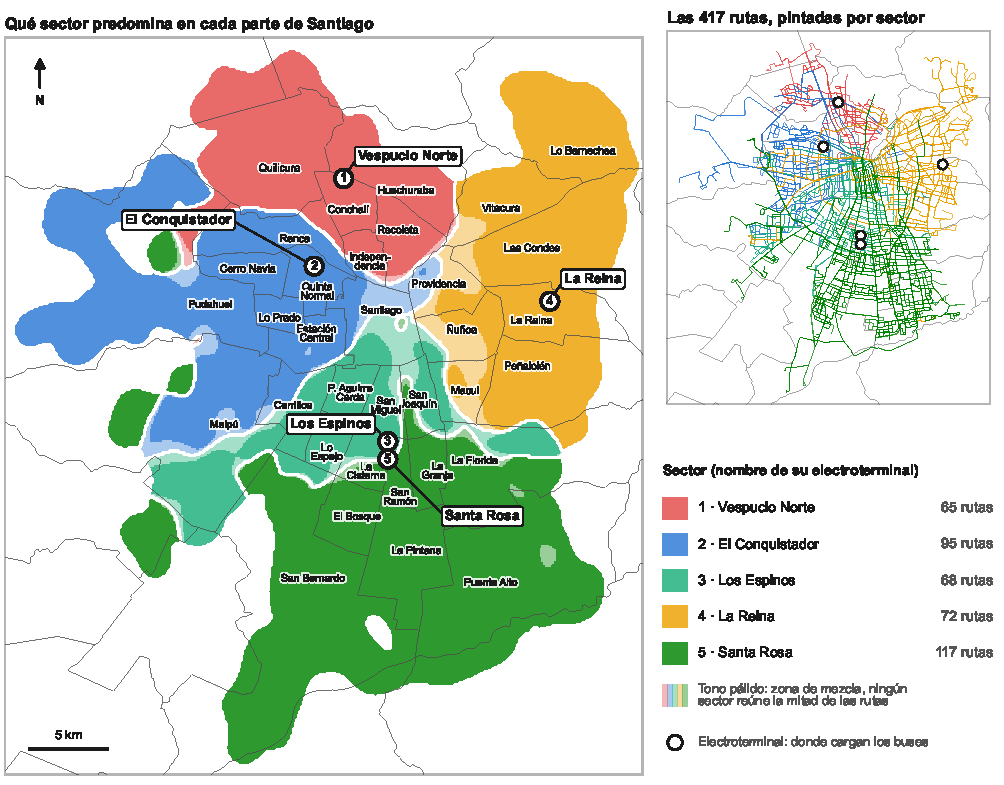
\includegraphics[width=0.84\linewidth]{mapa_sectores.pdf}
\caption*{\textbf{Los cinco sectores.} A la izquierda, cada parte de Santiago tiene el color del sector al que
pertenece la mayoría de las rutas que pasan por ahí. A la derecha están las rutas reales.}
\end{figure}

\newpage

\section{El método, en cuatro pasos}
\paso{1}{un primer plan rápido} Se recorren los viajes en orden de hora. Cada viaje se le da a un bus del
sector que esté libre, alcance a llegar y tenga batería. Si ninguno puede, se agrega un bus nuevo. Sale un
plan válido de \BusesBase{} buses (USD~\CostoBase{} al día). Es rápido pero «miope»: decide sin mirar lo que
viene después, así que sobran buses.

\paso{2}{mejorar el plan eliminando buses} Se toma un bus con pocos viajes y se intenta repartir todos sus
viajes entre otros 3 buses. Los cuatro forman un grupo, o «cuarteto». Esos 3 se sortean al azar entre los
buses compatibles: los del mismo sector que tienen libre la hora del viaje y alcanzan a llegar. Si el
reparto funciona, ese bus sale del plan. Esto se repite miles de veces, con grupos distintos, hasta que se
acaba el tiempo.

\paso{3}{recalcular las recargas} Cada vez que se cambia un grupo, un modelo matemático (resuelto con el
programa Gurobi) decide cuándo y dónde recarga cada bus del grupo, al menor costo de electricidad. Respeta
las baterías y los cargadores libres. Si no hay forma de cargar a tiempo, el cambio se descarta.

\paso{4}{auditar} Un verificador independiente revisa el plan final regla por regla: viajes, horarios,
batería, cargadores, estacionamientos y costo. Todos los planes pasaron sin errores.

\section{Cómo elegimos el método}
Probamos grupos de 2, 3, 4, 5 y 8 buses, más una mezcla que va agrandando el grupo. Comparamos dos formas de
elegir los grupos:
\begin{itemize}
  \item \textbf{Por ranking:} siempre los candidatos «más compatibles», como en la Entrega~2.
  \item \textbf{Al azar:} un sorteo entre todos los compatibles, repetido con 3 sorteos distintos para no
        depender de la suerte.
\end{itemize}
Todos corrieron con el mismo tiempo (10, 20 y 40 minutos) y en el mismo computador. Gana el más barato con
el mismo tiempo.

\section{Resultado: día laboral, 40 minutos}
\begin{minipage}[t]{0.655\linewidth}
\vspace{0pt}
\small
\begin{tabularx}{\linewidth}{@{}Xrrr@{}}
\toprule
Método & Buses & USD al día & Costo \\
\midrule
\FilasMetodos
\bottomrule
\end{tabularx}

\vspace{2pt}
{\footnotesize\color{gris} Los métodos al azar muestran el promedio de sus 3 sorteos.}
\end{minipage}\hfill
\begin{minipage}[t]{0.32\linewidth}
\vspace{0pt}
\begin{caja}[verdeclaro]{Ganan los cuartetos al azar}
\small
\BusesCuartetos{} buses y $-$\AhorroCuartetos\,\% de costo. Son \MenosBusesCuartetos{} buses y unos
USD~60.000 al día menos que el primer plan, y \MenosQueEntregaDos{} buses menos que lo entregado en la Entrega~2.
\end{caja}
\end{minipage}

\vspace{4pt}
\textbf{Elegir al azar es lo que más ayuda:} con tríos, duplica el ahorro. Con grupos de 5 o más el ahorro
cae, porque coordinar a tantos buses a la vez casi nunca resulta.

\end{document}
